% =====================================================================
%  G4b - Caliper SUSTAINED-LOAD scenario:
%  Request rate held at 200 TPS across all four round sizes; achieved
%  throughput stays at ~200 TPS while success rate degrades and average
%  latency rises as the chaincode world state grows.
%  Source: chapter4.tex Table tab:caliper, sustained columns.
% =====================================================================
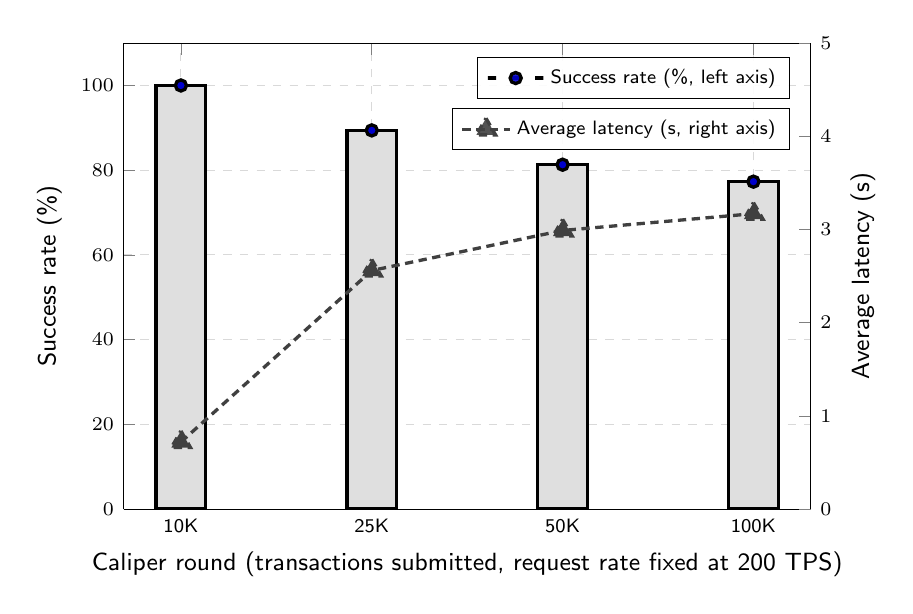
\begin{tikzpicture}
\begin{axis}[
    width=0.85\textwidth,
    height=7.5cm,
    axis y line*=left,
    xlabel={Caliper round (transactions submitted, request rate fixed at 200~TPS)},
    ylabel={Success rate (\%)},
    ymin=0, ymax=110,
    symbolic x coords={10K, 25K, 50K, 100K},
    xtick=data,
    bar width=18pt,
    grid=major,
    grid style={dashed, gray!30},
    legend style={at={(0.97,0.97)}, anchor=north east,
                  font=\sffamily\scriptsize, draw=black,
                  fill=white, fill opacity=0.90, text opacity=1},
    label style={font=\sffamily\small},
    tick label style={font=\sffamily\scriptsize},
]
\addplot+[ybar, fill=gray!25, draw=black, very thick] coordinates {
    (10K,   100.0)
    (25K,    89.4)
    (50K,    81.3)
    (100K,   77.3)
};
\addlegendentry{Success rate (\%, left axis)}
\end{axis}

\begin{axis}[
    width=0.85\textwidth,
    height=7.5cm,
    axis y line*=right,
    axis x line=none,
    ylabel={Average latency (s)},
    ymin=0, ymax=5,
    symbolic x coords={10K, 25K, 50K, 100K},
    xtick=data,
    legend style={at={(0.97,0.86)}, anchor=north east,
                  font=\sffamily\scriptsize, draw=black,
                  fill=white, fill opacity=0.90, text opacity=1},
    label style={font=\sffamily\small},
    tick label style={font=\sffamily\scriptsize},
    every axis plot/.append style={thick},
]
\addplot+[mark=triangle*, mark size=4pt, color=black!75, mark options={fill=black!75},
          densely dashed, very thick] coordinates {
    (10K,   0.72)
    (25K,   2.56)
    (50K,   2.99)
    (100K,  3.17)
};
\addlegendentry{Average latency (s, right axis)}
\end{axis}
\end{tikzpicture}
